\begin{Ueberlieferung}% 
{\textit{L}}Konzept:
 LH XXXVII 5 Bl. 57.
1 Bl. 4\textsuperscript{o}. 2~S.\\%
Cc 2, Nr. 836
\end{Ueberlieferung}
%
% \begin{Datierungsgruende}%
% Von Leibniz datiert.
% \end{Datierungsgruende}
%
\count\Afootins=1200
\count\Bfootins=1200
\count\Cfootins=1200
\vspace{8mm}
%\newpage
\pstart%
% [57~r\textsuperscript{o}]
\noindent[57~r\textsuperscript{o}] 1674. Parisiis.%
\newline%
Totum continuandi Motus \edtext{artificium in eo consistit,}{\lemma{artificium}\Bfootnote{\textit{(1)}\ est, \textit{(2)}\ in eo consistit, \textit{L}}} ut inveniatur ratio restituendi vim restituentem\protect\index{Sachverzeichnis}{vis restituens}, aliunde quam per restituendam. Itaque duae vires ita inter se invicem applicandae sunt, ut vis restituens rem suam agat separatim, compensatis omnibus, sans interesser  
la machine. Hoc vero admirabili quadam  ratione, sic fieri potest:
\pend 
%\vspace{1em}
%\pstart
%\centering
%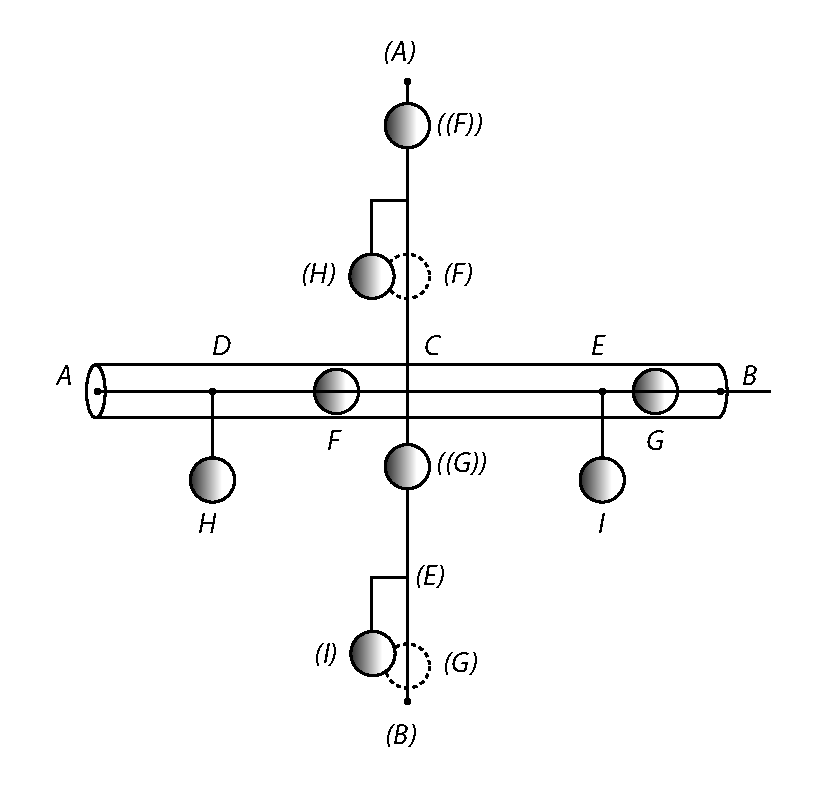
\includegraphics[trim = 0mm 6mm 0mm 5mm, clip, width=0.85\textwidth]{images/LH37,05_057r-d.pdf}\\
%\noindent \centering [\textit{Fig. 1}] 
%\pend
\pstart
%\begin{wrapfigure}{l}{0.57\textwidth}
%\vspace{-5mm} 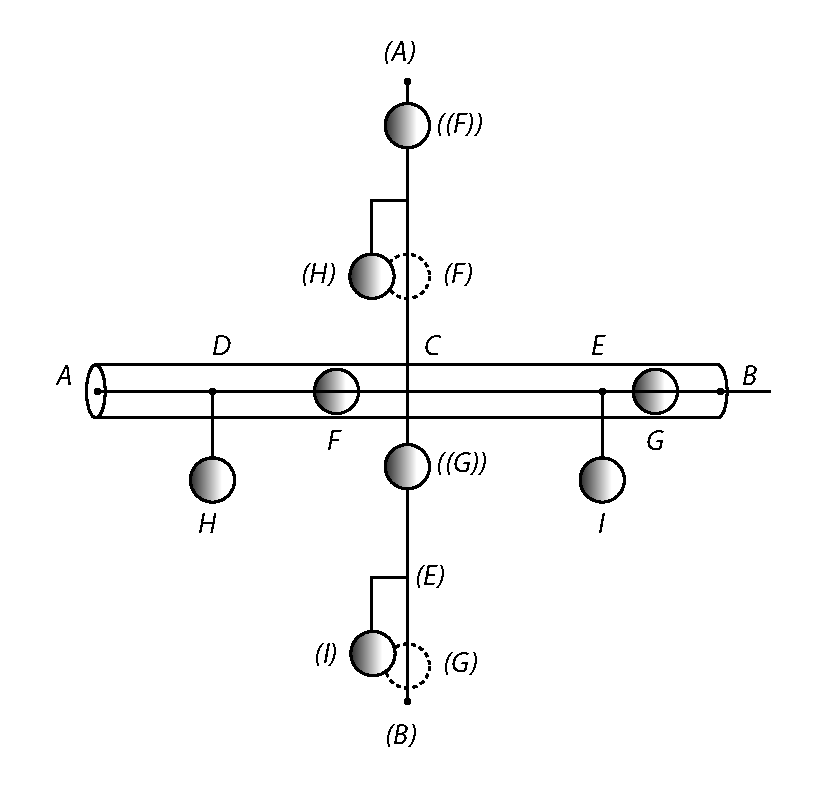
\includegraphics[trim = 6mm 6mm 3mm 0mm, clip, width=0.57\textwidth]{images/LH37,05_057r-d.pdf}\\
%\noindent \centering [\textit{Fig. 1}] 
%\end{wrapfigure}
\indent Esto canalis $AB$ mobilis circa centrum in medio $C$ quod tubum in duas dividit partes communicationem inter se non habentes. \edtext{Medietates $AC$,}{\lemma{Medietates}\Bfootnote{\textit{(1)}\ $AB$ \textit{(2)}\ $AC$, \textit{L}}} $BC$ subsectae sunto in duas  partes aequales $AD$, $DC$, vel $CE$, $EB$ in punctis $D$, $E$. Mobiles sint in  
\edtext{canali globi duo sic satis ponderosi, globus $F$}{\lemma{canali}\Bfootnote{\textit{(1)}\ pondera duo, pondus \textit{(2)}\ globi [...] globus  $F$
\textit{L}}}\protect\index{Sachverzeichnis}{globus} in medietate \edtext{$AC$, globus}{\lemma{$AC$,}\Bfootnote{\textit{(1)}\ pondus \textit{(2)}\ globus \textit{L} }} autem \edtext{$G$ in medietate}{\lemma{$G$}\Bfootnote{\textit{(1)}\ in ponder \textit{(2)}\ in medietate \textit{L}}} $CB$.%
\newline%
\hspace*{7,5mm}%
Ex punctis $D$, $E$ descendant pondera\protect\index{Sachverzeichnis}{pondus} $H$, $I$ lineis rigidis \edtext{sive regulis}{\lemma{}\Bfootnote{sive regulis \textit{erg.} \textit{L}}} $DH$, $EI$ circa centra, $D$, $E$, mobilibus affixa. Quod\-libet horum ponderum $H$, $I$ Elaterium\protect\index{Sachverzeichnis}{elaterium} in spiram\protect\index{Sachverzeichnis}{spira} si placet convolutum gestet; tantarumque sit virium pondus ut dum machina\protect\index{Sachverzeichnis}{machina} ex situ \edtext{$AB$ versus situm $(A)(B)$%
}{\lemma{$AB$}\Bfootnote{%
\textit{(1)}\ in %
\textit{(2)}\ versus situm %
\textit{(a)}\ $LM$ %
\textit{(b)}\ $(A)(B)$ \textit{L}}} \edtext{tendit in situm $(B)$ \textlangle ob pondus\textrangle\ $G$ remotiorem in centro quam $F$, tunc pondus $I$ nisu}{\lemma{tendit}\Bfootnote{\textit{(1)}\ $B$ scilicet tendente in $M$ pondus nisu suo $I$, \textit{(2)}\ ob pondus $G$ remotius a centro quam $F$, pondus nisu suo $I$  \textit{(3)}\ in situm [...] nisu suo \textit{L}\ }} suo contra canalem rigidum $CB$, cui scilicet inter descendendum appropinquat, spiram suam nullo negotio involvat in se, sive tendat. At ubi in situm perpendicularem \edtext{$(A)(B)$ vel paulo citeriorem}{\lemma{$(A)(B)$}\Bfootnote{\textit{(1)}\ paulo scilicet \textit{(2)}\ vel paulo citeriorem \textit{L}}} aut (ob accelerationem\protect\index{Sachverzeichnis}{acceleratio} descensus \edtext{si nullo alio motu oneretur}{\lemma{}\Bfootnote{si nullo alio motu oneretur \textit{erg.} \textit{L}}}) paulo ulteriorem, pervenerit, liberetur spira (impactu quodam aliterve, cessante si placet contactu canalis).  Seque restituens pondus $G$ nunc translatum in locum $G$, inde sursum pellat in locum $((G))$. 
\pend 
\pstart
\centering
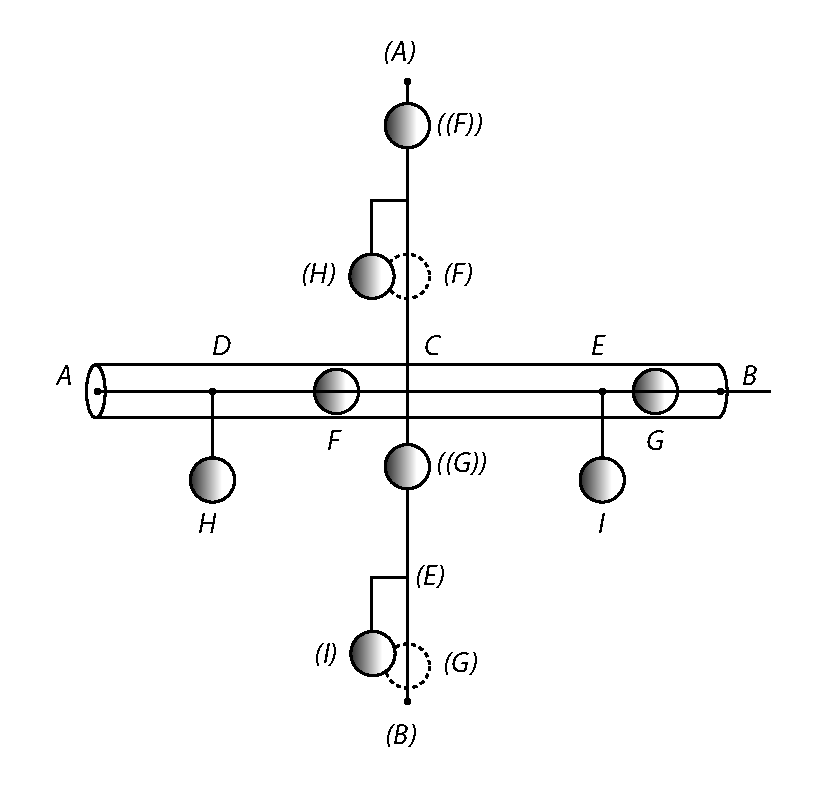
\includegraphics[trim = 0mm 6mm 0mm 5mm, clip, width=0.82\textwidth]{images/LH37,05_057r-d.pdf}\\
\noindent \centering [\textit{Fig. 1}] 
\pend
\vspace{1.5em}
\pstart
Eodem
\setline{1}\edtext{tempore dum brachium $B$ descendit in $(B)$}{\lemma{tempore}\Bfootnote{%
\textit{(1)}\ spira ponderis $H$ contra brachium $AC$ nitens %
\textit{(2)}\ dum [...] in $(B)$ \textit{L}}}
\edtext{brachium\protect\index{Sachverzeichnis}{brachium} $A$ ascendet ad $(A)$}{\lemma{brachium $A$}\Bfootnote{%
\textit{(1)}\ descendet in $A$ %
\textit{(2)}\ ascendet ad $(A)$ \textit{L}}}
et pondus $H$ tendens ad locum $(H)$ nitensque eodem modo contra canalem $AC$, spiram suam tendet,
quae denique eodem tempore quo inferior liberabitur,
et dum inferior pilam\protect\index{Sachverzeichnis}{pila} $(G)$ elevat ad $((G))$ pilam $(F)$ elevabit ad $((F))$.
\pend 
%\newpage
\pstart
Ponendo jam lineam $(A)(B)$ esse nonnihil inclinatam ad horizontem, et ut minimum certumque dicamus, restitutionem spirae fieri, $(B)$ nondum omnino ad perpendiculum delato, ac proinde $(G)$ dexteriore $((F))$ sinisteriore machina retrogradetur ob pondus $((F))$ remotius a centro $C$ quam pondus $(G)$ eademque omnia evenient quae \edtext{ante: latere tantum contrario substituto}{\lemma{ante:}\Bfootnote{\textit{(1)}\ continuis reciprocationibus \textit{(2)}\ latere [...] substituto. \textit{L}}}. Eaeque reciprocationes sine fine repetentur. Quodsi velis machinam in eundem continuo sensum ire hoc efficiemus \edtext{si ipsa motus acceleratione canalis}{\lemma{si}\Bfootnote{\textit{(1)}\ machina \textit{(2)}\ ipsa [...] canalis \textit{L}}} in $(A)(B)$ ultra perpendicularem $B$ descendendo nonnihil evagetur, ita ut $(B)$ veniens a $B$ fiat sinisterior $(A)$ veniens ab $A$ \edtext{dexterior. Sed}{\lemma{dexterior.}\Bfootnote{\textit{(1)}\ Ita enim \textit{(2)}\ Sed \textit{L}}} quoniam non est fidendum accelerationi\protect\index{Sachverzeichnis}{acceleratio} \edtext{si machina}{\lemma{si}\Bfootnote{%
\textit{(1)}\ motus %
\textit{(2)}\ machina \textit{L}}}
\edtext{forte ad opus quoddam}{\lemma{forte}\Bfootnote{\textbar\  labore \textit{gestr.} \textbar\ ad opus \textit{L}}}
applicanda
\edtext{sit, ubi}{\lemma{sit,}\Bfootnote{\textit{(1)}\ ideo ab \textit{(2)}\ ubi \textit{L}}} acceleratio detrimentis obstaculorum compensatur, \edtext{ideo consultissimum est}{\lemma{ideo}\Bfootnote{\textit{(1)}\ satis est \textit{(2)}\ consultissimum est \textit{L}}} canalem $AB$, ab alio simili similiterque \edtext{formato ad}{\lemma{formato}\Bfootnote{\textit{(1)}\ ab \textit{(2)}\ ad \textit{L}}} angulos rectos intersecari. Restitutiones autem non nisi in situ perpendiculari fieri imo non video quid impediat plures adhuc adhiberi canales; semper enim fiet hoc modo \edtext{ut pilae\protect\index{Sachverzeichnis}{pila} sinistrae}{\lemma{ut}\Bfootnote{\textit{(1)}\ pondera sinistra \textit{(2)}\ pilae sinistrae \textit{L}}} $F$ sint propiores centro, dextrae $G$ remotiores.
[57~v\textsuperscript{o}]
\pend
\pstart%
Quod si metuamus ne pondera\protect\index{Sachverzeichnis}{pondus}  $I$, $H$, aliaque gyrationibus circa  
centra $D$, $E$ etc. factis se mutuo impediant, potest fieri, ut diversi canales et duobus \edtext{perpendiculares primis, non sint}{\lemma{perpendiculares}\Bfootnote{\textit{(1)}\ non sint \textit{(2)}\  primis, non sint \textit{L}}} ut in eodem plano. \edtext{Sufficietque duos}{\lemma{Sufficietque}\Bfootnote{\textit{(1)}\ duosque \textit{(2)}\ duos \textit{L}}} quoslibet canales perpendiculares inter se in eodem esse plano. Quod si vim omnem hac machina\protect\index{Sachverzeichnis}{machina} possibilem quaeramus[,]
 plures ejusmodi rotae in unum cylindrum linea rigida per omnium centra transeuntes jungi possunt. 
\pend 
\pstart 
Elateria\protect\index{Sachverzeichnis}{elaterium} autem pondera pilas\protect\index{Sachverzeichnis}{pila} tantae magnitudinis esse posse manifestum est, ut machina\protect\index{Sachverzeichnis}{machina} molendini\protect\index{Sachverzeichnis}{molendinum} locum supplere possit.
\pend 
\pstart 
Potest et elegantius res ita institui, ut circa centra $D$, $E$ radios $EI$, $DH$ sint Epicycli cavi, in quibus pondera $I$, $H$ et ipsa in pilas tornata circumeant spiramque in extremo $B$ fixam tendant, ita, ut ubi in Epicyclo \edtext{ad debite oppositum locum}{\lemma{ad}\Bfootnote{\textit{(1)}\ debitum quendam \textit{(2)}\ debite oppositum locum \textit{L}}} venere tangendo aliquid, spiram denuo restituant. Hoc modo illud quoque commodum habebitur ut spira\protect\index{Sachverzeichnis}{spira} quae pondus elevavit, et sustineat, donec adsit tempus tendendae rursus spirae, ubi et nulla opus restitutione. 
\pend
% \newpage%
\vspace*{1.0em}% PR: Abstand rein provisorisch !!!!
\pstart%
\noindent%
1678 Hanoverae mense Majo.
\newline%
\noindent%
\edtext{Dudum}{\lemma{Dudum}\Bfootnote{\textit{(1)}\ nota \textit{(2)}\ sciebam \textit{L}}}
sciebam inesse paralogismum,
quem nunc manifeste \edtext{video. Ajo igitur}{\lemma{video.}\Bfootnote{%
\textit{(1)}\ Primum %
\textit{(2)}\ Elateria tollamus, atque idem solis ponderibus efficiamus. Sint $H.$ $I$ pondera %
\textit{(3)}\ Manifestum est %
\textit{(4)}\ Ajo igitur \textit{L}}}
\edtext{si Elastrum $I$ tendendum}{\lemma{si}\Bfootnote{%
\textit{(1)}\ Elaterium %
\textit{(2)}\ Elastrum \textbar\ $I$ \textit{erg.} \textbar\ tendendum \textit{L}}}
tantarum est virium, ut pondus
\edtext{$G$}{\lemma{$G$}\Bfootnote{\textit{erg. L}}}
in canali elevare possit, ubi ad situm prope perpendicularem descendit,
et si pondus $I$ tantarum est virium, ut Elastrum hoc tendere possit,
tunc omnibus sibi relictis nullum fore motum,
\edtext{seu canalem}{\lemma{seu}\Bfootnote{\textit{(1)}\ corpus \textit{(2)}\ canalem \textit{L}}}
$CB$ non descensurum in $C(B)$.
Quod ut appareat
\edtext{fingamus non continue pondus}%
{\lemma{fingamus}\Bfootnote{\textit{(1)}\ canalem \textit{(2)}\ non continue pondus \textit{L}}}
$I$ circa centrum $E$ esse mobile,
sed nonnihil vel perexiguum tempus canalem solum descendere,
ponderibus $I$ et $H$ manentibus firmis.
Ajo tunc nullum fore motum, quod ostendo, quia tunc descendente canali $CB$ versus $C(B)$
pondus $H$ nimis alte elevabitur pariter ac pondus $I$, et exigua vi magnam nobis vim parabimus;
quod est absurdum. Major autem utique vis ponderis
quia Elaterium fortius ponderibus descendentibus in canali,
et pondera $I.$ $H$ fortiora elateriis quae debent tendere.
Quod cum non fiat in tempore, nec fiet in tempore infinite
\edtext{parvo, seu}{\lemma{parvo,}\Bfootnote{%
\textit{(1)}\ id est %
\textit{(2)}\ si scili %
\textit{(3)}\ seu \textit{L}}}
non fiet etsi continue simul incedant.
Quia quolibet momento paratur vis major quam quae adhibetur; seu effectus potentior causa.
Elegans est hoc exemplum quo ostenditur, homines etiam ingeniosissimos, et maxime valentes imaginandi potestate,
errorem hunc non deprehensuros nisi metaphysicis principiis, nempe rationibus
\edtext{circa potentiam,}{\lemma{circa}\Bfootnote{\textit{(1)}\ vim \textit{(2)}\ potentiam, \textit{L}}}
et infinite parva adhibitis.
Nam qui id non facit, is profecto nunquam deteget hunc paralogismum.
\pend
\count\Afootins=1500
\count\Bfootins=1500
\count\Cfootins=1500
